\section{Eye Tracking Technology} \label{sec:bt/ET_tech}

Eye-tracking systems have existed in some way since the late 1800s \cite{holmqvist2011}. The first occurrences included bite-bars to ensure still head positions and mechanical rings attached to the eyeball. More modern techniques are based on electromagnetic inductance in a specially constructed lens, others directly on the electromagnetic activation of the extraocular muscles. The latter is more commonly known as electrooculography and is still present today in some systems. Ever since the appearance of the pupil- and corneal reflection method, the nature of which will be explained shortly, that has been the primary approach in all modern eye-tracking systems. 

The dominance of the pupil- and corneal reflection method comes from its minimally intrusive manner, as it allows for precise and accurate gaze estimation from a video recording of the user's eye movements. The hardware of such eye-trackers consists of at least one high-resolution and high-frequency camera, accompanied by one or more infrared light sources directed at the user. These light sources will produce a visible reflection on the cornea, which, together with the pupil, serves as reference points to determine gaze direction and head position. An example is illustrated in figure \ref{fig:bt_pupil_corneal_reflection}. Positions of reference points in the image are determined using computer vision algorithms. A calibration process is initially required to provide the system with known reference point relationships corresponding to known gaze points in the tracking area. The rest of the tracking area is then interpolated between calibration points. While even one camera and one light source provide a reasonably accurate gaze position as long as the head is fairly still, more cameras and infrared sources can be used to relax the constraints on head movement and calibration \cite{holmqvist2011}. 

\begin{figure}[h]
    \centering
    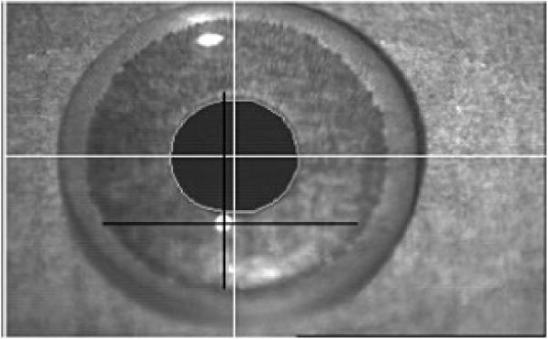
\includegraphics[width=0.8\textwidth]{figures/bt_pupil_corneal_reflection.png}
    \caption{Demonstration of pupil- and corneal reflection. The white and black crosses correspond to the point indentified as the pupil and corneal reflection centers, respectively.}
    \source{\textcite{holmqvist2011}}
    \label{fig:bt_pupil_corneal_reflection}
\end{figure}

All eye-tracking methods suffer from a deficiency in degrading estimation with large gaze angles. In the extremes, the corneal reflection is often lost. Eye-trackers utilizing the pupil- and corneal reflection method rarely support gaze angles beyond 40$^{\circ}$ in the horizontal direction and 25$^{\circ}$ in the vertical direction. Given the viewing distance, $d$ and the gaze angle $\theta$, the corresponding unit $x$ in the stimulus space is given by equation \ref{eq:bt_stimulus_deg_rel}. Note, however, that this relationship only holds when $\theta$ is small, i.e., when the user looks at points close to the tracker camera. As such, the same visual angle $\theta_1$ may result in different displacements ($x_1$ and $x_2$) on the stimulus for progressively larger gaze angles, as illustrated in figure \ref{fig:bt_stimulus_deg_rel}.

\begin{equation}
    \tan{\dfrac{\theta}{2}} = \dfrac{x}{d}
    \label{eq:bt_stimulus_deg_rel}
\end{equation}

% Remote eye tracking
%     - Tracking range and visual boxes
% \newpage

\begin{figure}[h]
    \centering
    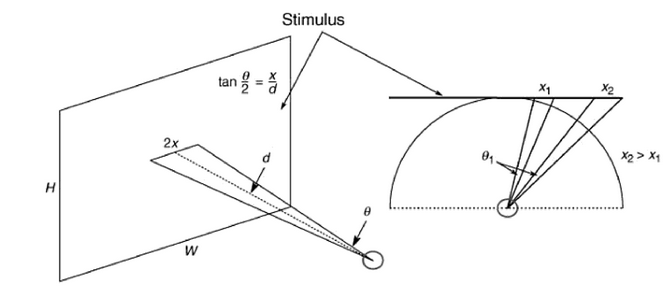
\includegraphics[width=0.8\textwidth]{figures/bt_angle_stimulus_relationship.png}
    \caption{Geometric relationship between stimulus and degrees of visual angle.}
    \source{\textcite{holmqvist2011}}
    \label{fig:bt_stimulus_deg_rel}
\end{figure}

All eye trackers come with a given sampling rate, and the speed at which data is recorded is typically the primary contributor to its price. Considering eye movements as an oscillating behavior, one can use the Nyquist-Shannon sampling theorem to argue that a sampling frequency at least twice as large as the largest frequency component of the signal is required. It means that a sampling rate of 300Hz is necessary to estimate the movements of micro-saccades, which can oscillate at 150Hz. Still, for most use cases, it is often sufficient only to evaluate the more significant eye movements such as saccades, fixations, and smooth pursuits, which are not oscillating and subsequently require less strict sampling rates. 

% Even so, as was detailed in section \ref{sec:bt_TheOculomotorSystem}, saccades can occur with durations as short as 30ms. 

% \newpage

% Sampling rate considerations
%     - Latency
%     - Saccadic velocity
%     - Measures of data quality
%         - Accuracy
%         - Precision

